\documentclass[final]{beamer}
\usepackage{natbib}
\usepackage{lmodern}
\usepackage[utf8]{inputenc}
\usepackage[T1]{fontenc}
\usepackage[ngerman]{babel}
%\usepackage{pstricks}
%\usepackage{pst-node}
%\usepackage[all]{xy}
\def\newblock{\hskip .11em plus .33em minus .07em}
\title[Masterarbeit - Kolloquium]{Entwurf von Algorithmen zur Lösung von Objektverschiebungsproblemen \\ \small Kolloquium}   
\author{Maximilian Mühlfeld} 
\date{\today} 
\usepackage{multimedia}
%\usepackage{media9}
\usepackage{hyperref}
\usepackage{beamerthemesplit} % kam neu dazu
\setbeamercovered{invisible}
% Alternativ kann man auch das Usetheme Warsaw nutzen
\usetheme{Warsaw}
\usepackage[rightcaption]{sidecap}
\setbeamerfont{footline}{size=\tiny}
\AtBeginSection[]{
\begin{frame}<beamer>
\frametitle{Inhalt} %oder wie auch immer die Folie benannt sein soll
\tableofcontents[currentsection,currentsubsection,currentsubsubsection,hideothersubsections]
\end{frame}
}
\begin{document}


\begin{frame}
\titlepage
\end{frame} 

\begin{frame}
\frametitle{Inhaltsverzeichnis}
\scriptsize
\tableofcontents
\end{frame} 


\section{Einleitung} 
\begin{frame}
\frametitle{Ziel}
\begin{figure}
\includegraphics[scale=0.1]{../thesis/mixedriddle}
\includegraphics[scale=0.1]{../thesis/boxriddle}
\end{figure}
Lösen von Verschiebungsproblemen bei gegebener Startkonfiguration und Zielposition eines Objektes.
\end{frame}


\begin{frame}
\frametitle{Motivation: Industrieroboter}
Industrieroboter werden meist nur in statischer Umgebung genutzt und eingerichtet mit absolut getrennten Arbeitsbereichen, da die Konfiguration der Roboterbahn somit simpel bleibt.\\
Idee:
\begin{itemize}
\item Mehrere Roboterarme parallel im selben Arbeitsraum.
\item Endeffektorwegplanung dynamisch mithilfe von Objekterkennung.
\end{itemize}
\end{frame}

\begin{frame}
\frametitle{Motivation: Automatisiertes Rätselerstellen}
Automatisches Testen von  Rätseln auf Lösbarkeit.
\begin{itemize}
\item Ermöglicht das Erstellen komplett zufälliger Rätsel ( z.b. im Rahmen eines Spieles ).
\item Erlaubt bei Erweiterung um mehrere Zielobjekte das Lösen von Puzzles mit vorgegebenem Endzustand.
\end{itemize}
\end{frame}

\section{Lösungsansätze und Grundlagen}
\begin{frame}
\frametitle{Ideen}
\begin{itemize}
\item Suche auf einem komplett definiertem Raster.
\item Schrittweise suchen nach einer besseren Konfiguration bis zur Zielkonfiguration mit/ohne Raster.
\item Einteilen des Raumes in Zellen und diese als Suchraum nutzen.
\end{itemize}
\end{frame}

\begin{frame}
\frametitle{Abstraktion:Objekte}
\begin{itemize}
\item Objekte werden als konvex angenomen.
\item Jedes Objekt ist durch einen Angelpunkt und der geordneten Liste seiner Eckpunkte definiert.
\item Je nach gewählter Repräsentation kann der Kantenzug des Objektes vorausberechnet mitgeliefert werden.
\end{itemize}
\begin{figure}
\centering
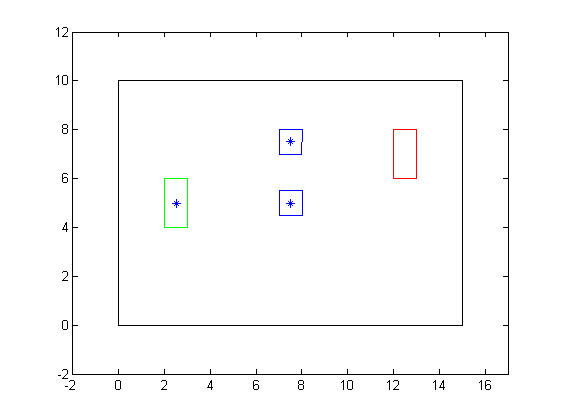
\includegraphics[scale=0.3]{../thesis/riddle2}
\end{figure}
\end{frame}

\begin{frame}
\frametitle{Abstraktion:Zellen}
\begin{itemize}
\item Zellen sind durch die Verlängerung der Kanten der Objekte begrenzt.
\item Jede Zelle ist definiert durch ihre Lage zu ALLEN Kanten der Objekte.
\end{itemize}
\begin{figure}
\centering
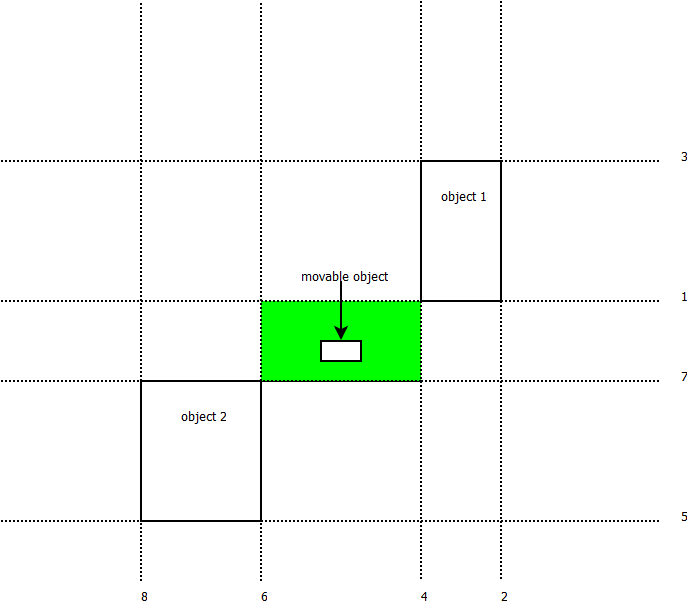
\includegraphics[scale=0.2]{../thesis/cellDivision}
\end{figure}
\end{frame}


\begin{frame}
\frametitle{Abstraktion:Konfiguration}
\begin{itemize}
\item Angelpunkte aller Objekte zusammen mit deren Drehwinkeln ergibt die momentane Konfiguration.
\end{itemize}
\begin{figure}
\centering
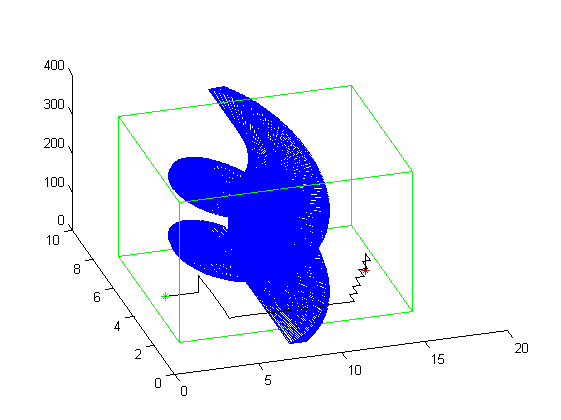
\includegraphics[scale=0.4]{../thesis/pathConfig}
\end{figure}
\end{frame}

\begin{frame}
\frametitle{Definiertes Raster}
\begin{figure} 
\centering
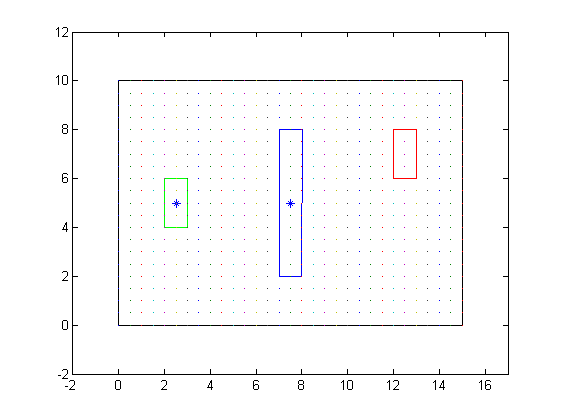
\includegraphics[scale=0.4]{../thesis/plotGridRot}
\end{figure}
\end{frame}

\begin{frame}
\frametitle{Definiertes Raster}
Für ein komplett definiertes Raster aller Konfigurationen muss jede mögliche Kombination berechnet werden.\\
Mit nur zwei Objekten ( ein Hauptobjekt und ein bewegliches Hindernis ) auf einem 10x10 Raster folgt für die Anzahl an Kombinationen:
\begin{align*}
N_{conf} &= (10*10*360)^2 \\
	&=   1296000000\\
	&= 1.296 \cdot 10^9\\
\end{align*}
TODO: tolle beispiele auf Zettel wieviel Speicher/Zeit benötigt
\end{frame}



\begin{frame}
\frametitle{Schrittweise aufbauen des Suchraumes mit Raster}
Anstelle das komplette Raster zu erstellen, werden immer nur die Knoten erstellt, die für den nächsten Schritt benötigt werden.
\begin{itemize}
\item Suchalgorithmen wie A$^\star$/Djikstra erlauben das generieren der Randknoten zur Laufzeit.
\item Verringert die Menge an benötigten Knoten enorm im Vergleich zum komplett definiertem Raster.
\end{itemize}
\end{frame}

%\begin{frame}
%\frametitle{Schrittweise aufbauen des Suchraumes mit Raster}
%\begin{figure}
%\centering
%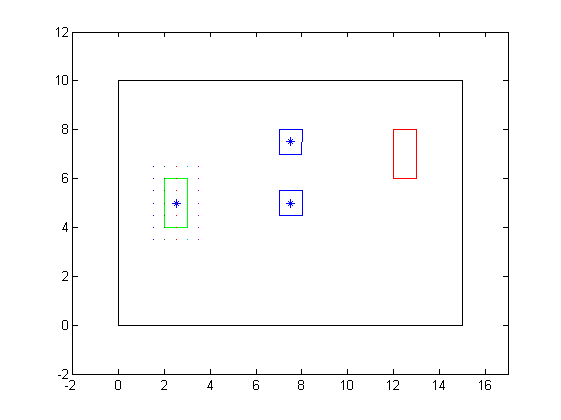
\includegraphics[scale=0.4]{../thesis/plotRimGrid}
%\end{figure}
%\end{frame}


\begin{frame}
\frametitle{Schrittweise aufbauen des Suchraumes ohne Raster}
Wir entfernen das Raster und erhalten dadurch eine unendliche Menge an möglichen Konfigurationen.
\begin{itemize}
\item Genaueres Bewegen der Objekte möglich durch exaktere Positionierung.
\item Die Anzahl der Knoten auf dem Pfad Ergebnispfad ist geringer 
\end{itemize}
\end{frame}
%
%\begin{frame}
%\frametitle{Schrittweise aufbauen des Suchraumes ohne Raster}
%\begin{figure}
%\centering
%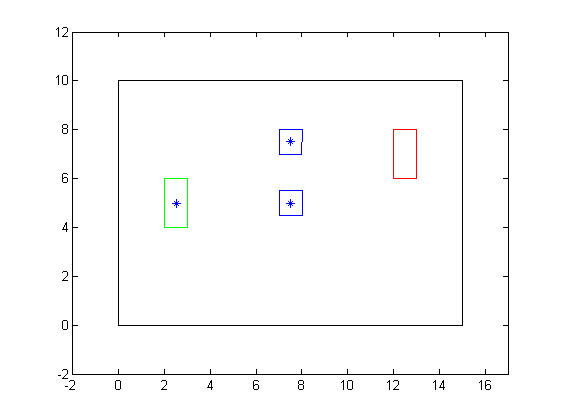
\includegraphics[scale=0.3]{../thesis/riddle2}
%\end{figure}
%\end{frame}


\begin{frame}
\frametitle{Einteilung des Raumes in Zellen}
Wir fügen eine Einteilung des Raumes in Zellen hinzu, welche zwar die Menge an Konfiguration reduziert, jedoch nicht die Genauigkeit.
\begin{itemize}
\item Zellen erlauben das Zusammenfassen von vielen Konfigurationen zu einem Punkt im Konfigurationsraum.
\item Die Zahl der Knoten die erstellt werden ist abhängig von der Zahl der Objekte, und nicht mehr von der gewünschten Genauigkeit.
\end{itemize}
\end{frame}

\begin{frame}
\frametitle{Schrittweise aufbauen des Suchraumes mit Zellen}
\begin{figure}
\centering
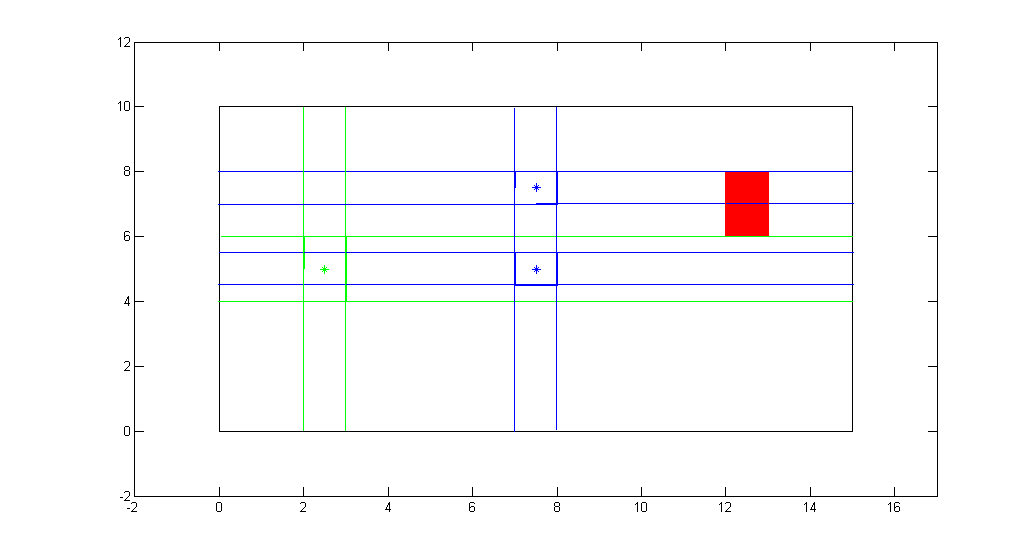
\includegraphics[scale=0.3]{../thesis/cellRiddle}
\end{figure}
\end{frame}

\begin{frame}
\frametitle{Schrittweise aufbauen des Suchraumes mit Zellen}
\begin{figure}
\centering
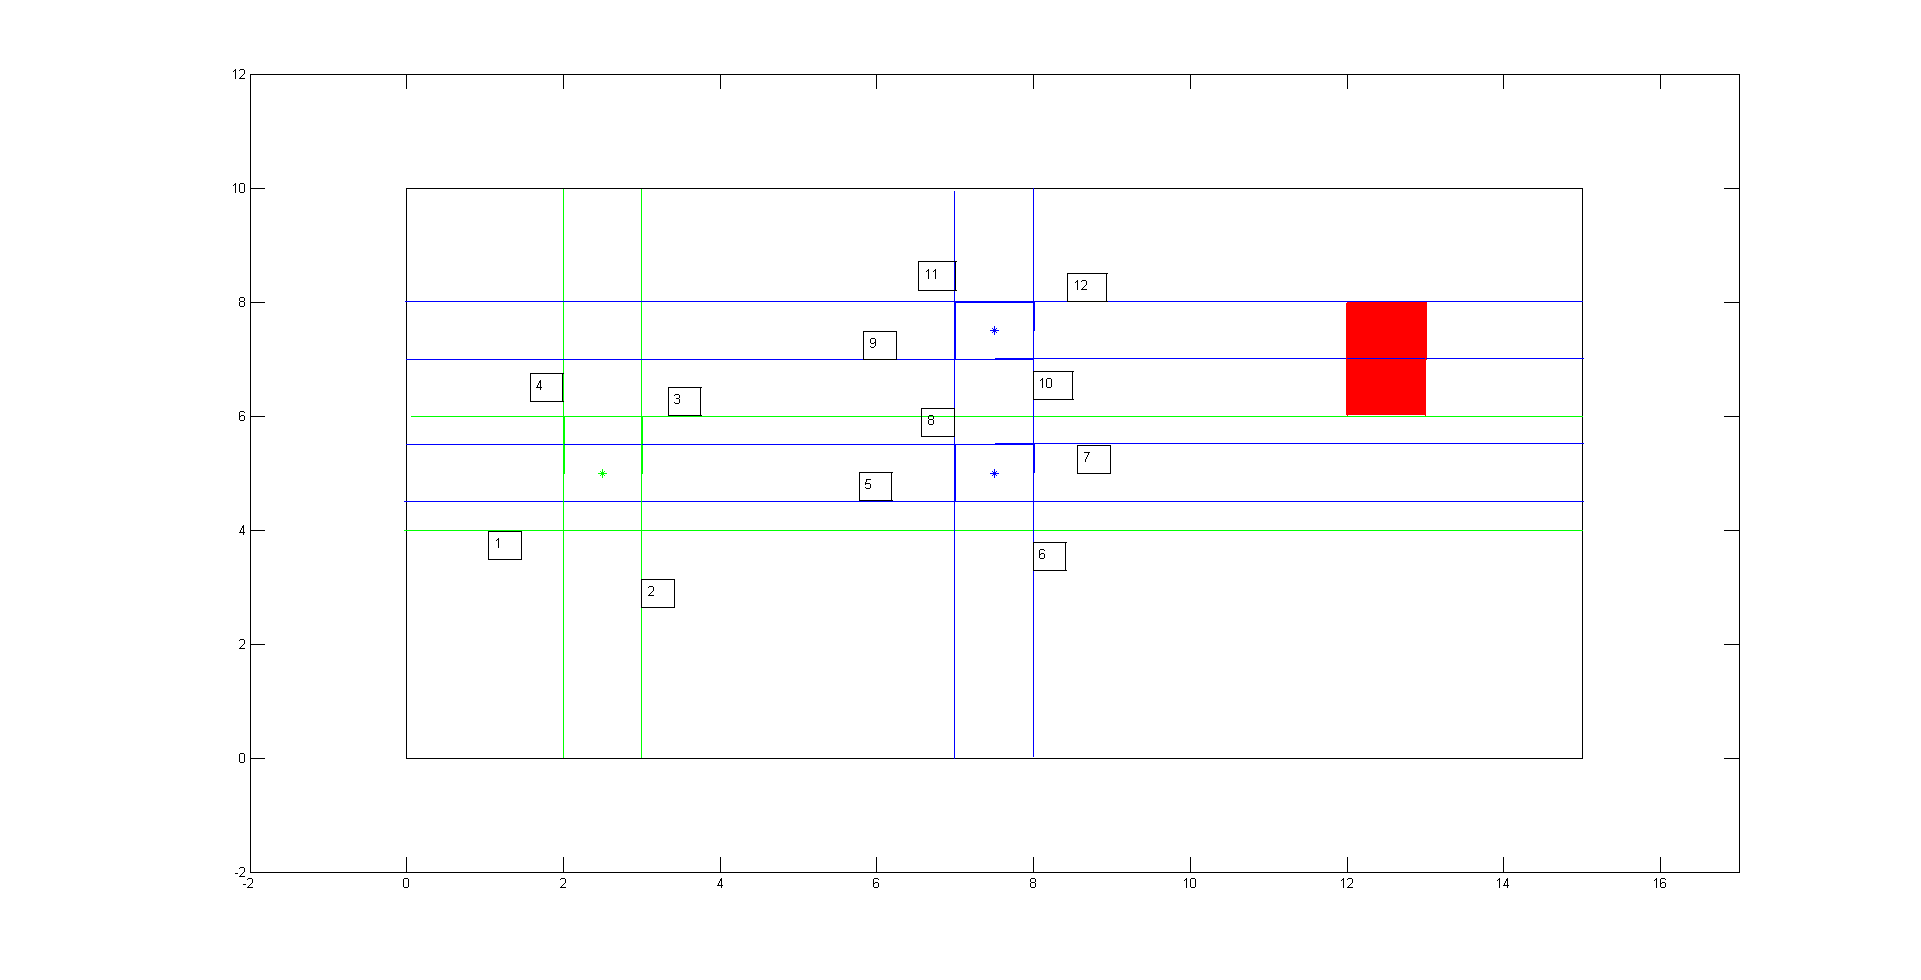
\includegraphics[scale=0.175]{../thesis/cellRiddleNumbered}
\end{figure}
\end{frame}


\section{Kantenrepräsentation mit Vektoren}
\begin{frame}
\frametitle{Kanten als Vektoren}
Da die Objekte aus sortierten Listen der Ecken bestehen, sind die Vektoren der Kanten einfach zu berechnen aus der Differenz der Eckpunkte. Hierfür wird keine Veränderung der Objekte benötigt.
\end{frame}

\begin{frame}
\frametitle{Kollisionsberechnung mittels Konvexer Hülle I }
Aufstellen der Konvexen Hülle aus den Ecken des momentan bewegten Objektes und allen anderen.
\begin{figure}
\centering
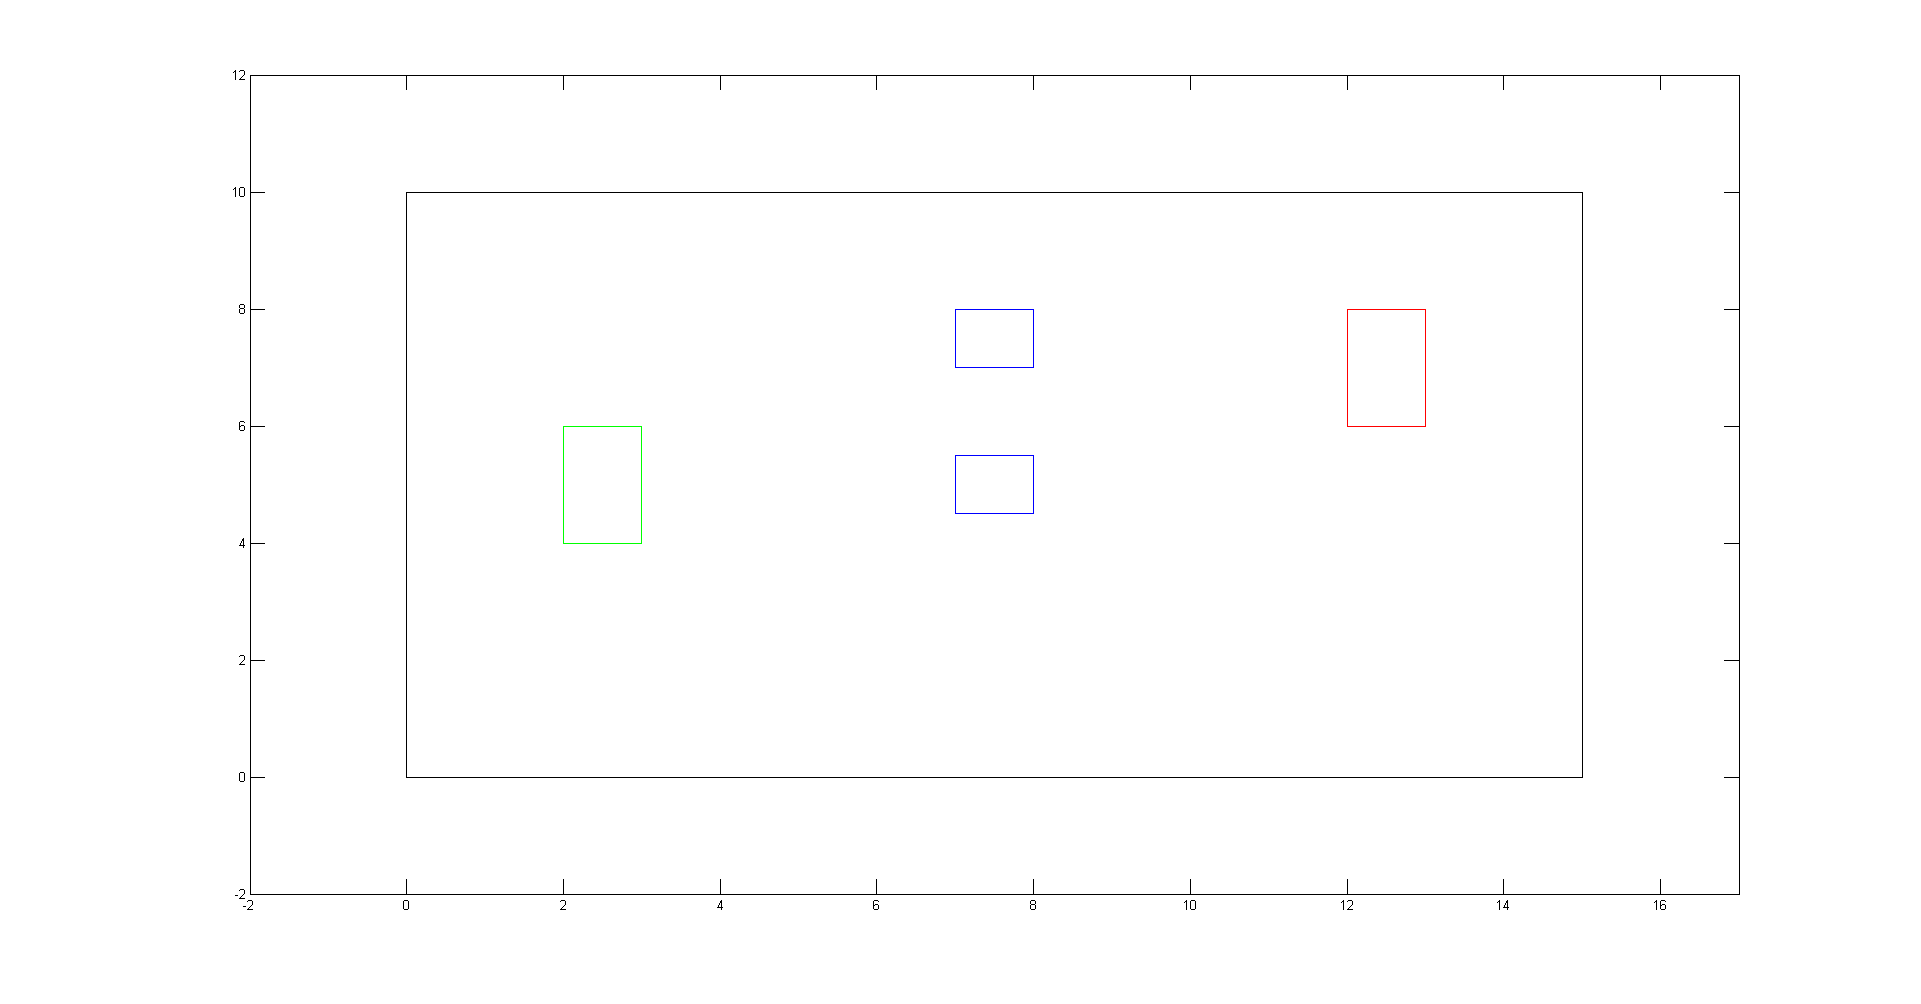
\includegraphics[scale=0.1]{../thesis/riddleWoHull}
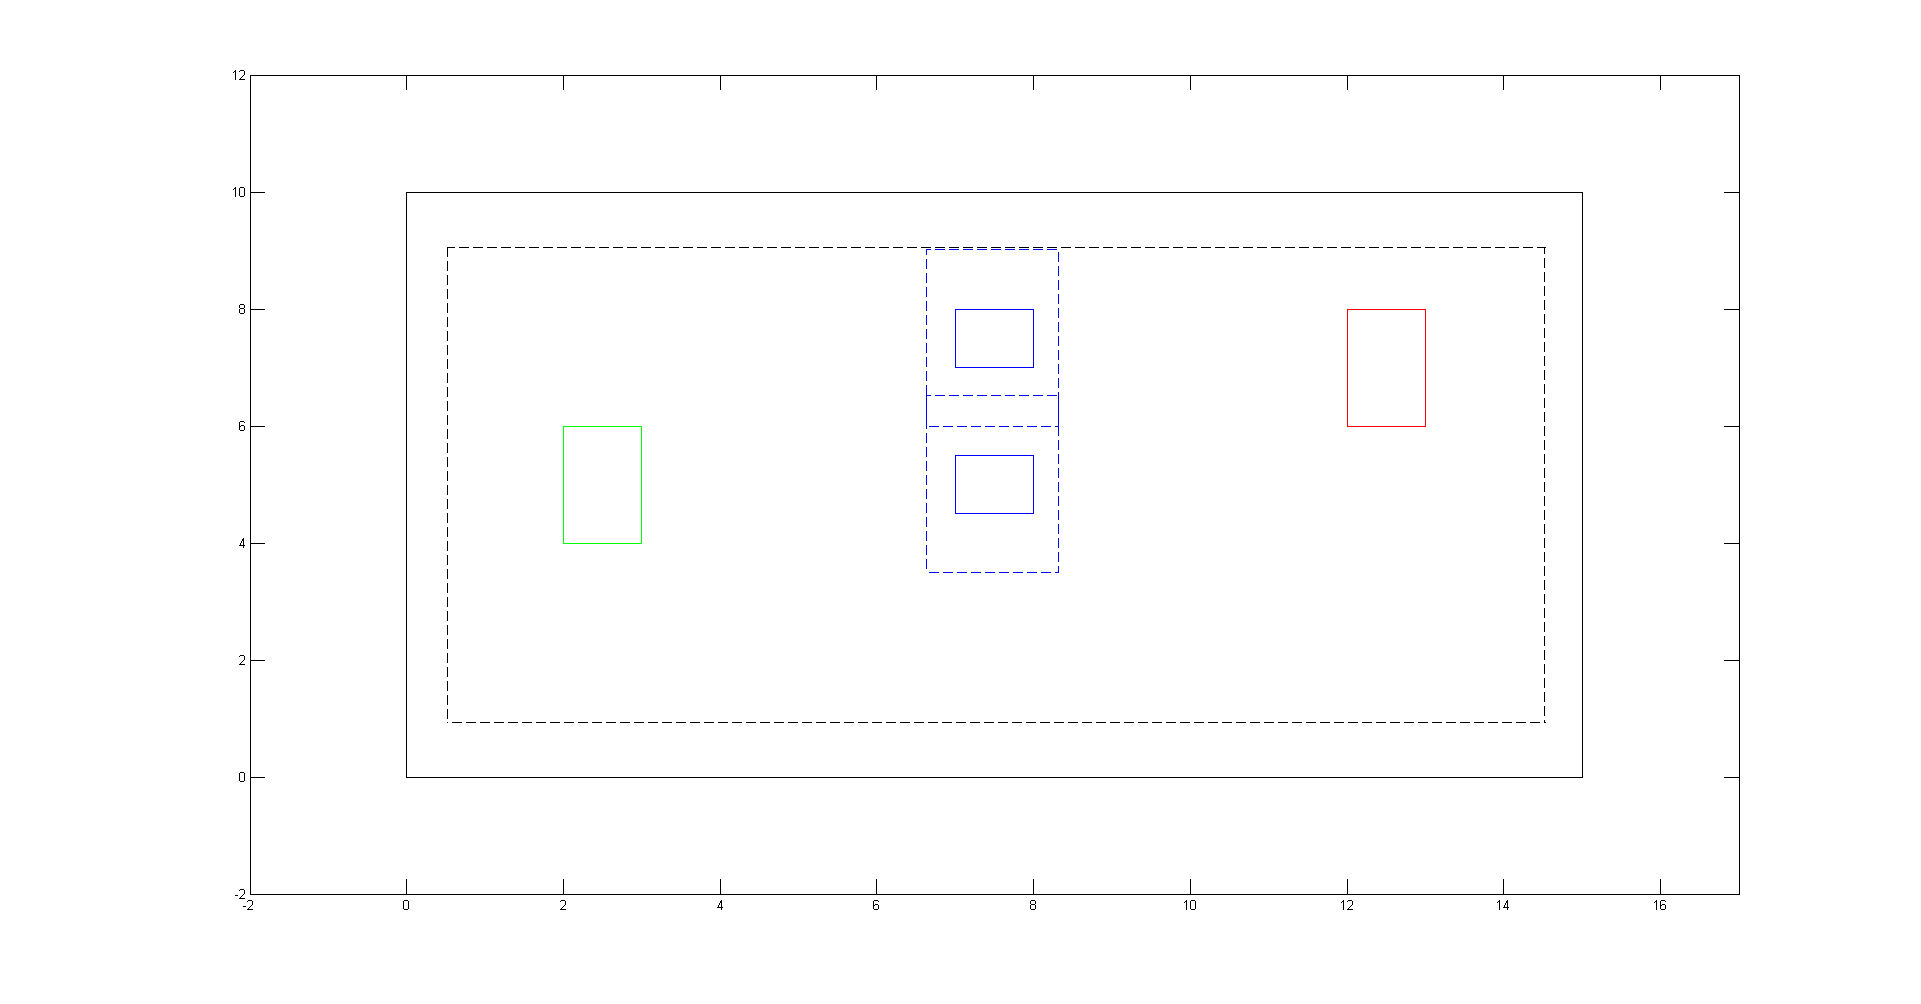
\includegraphics[scale=0.1]{../thesis/riddleWHull}
\end{figure}
\end{frame}

%\begin{frame}
%\frametitle{Kollisionsberechnung mittels Konvexer Hülle II}
%Der Vektor bestehend aus der Objektmitte als Aufpunkt und dem Richtungsvektor der Bewegung wird nun auf Schnittpunkte mit den Berechneten Vektoren der Konvexen Hüllen überprüft.
%\begin{figure}
%\centering
%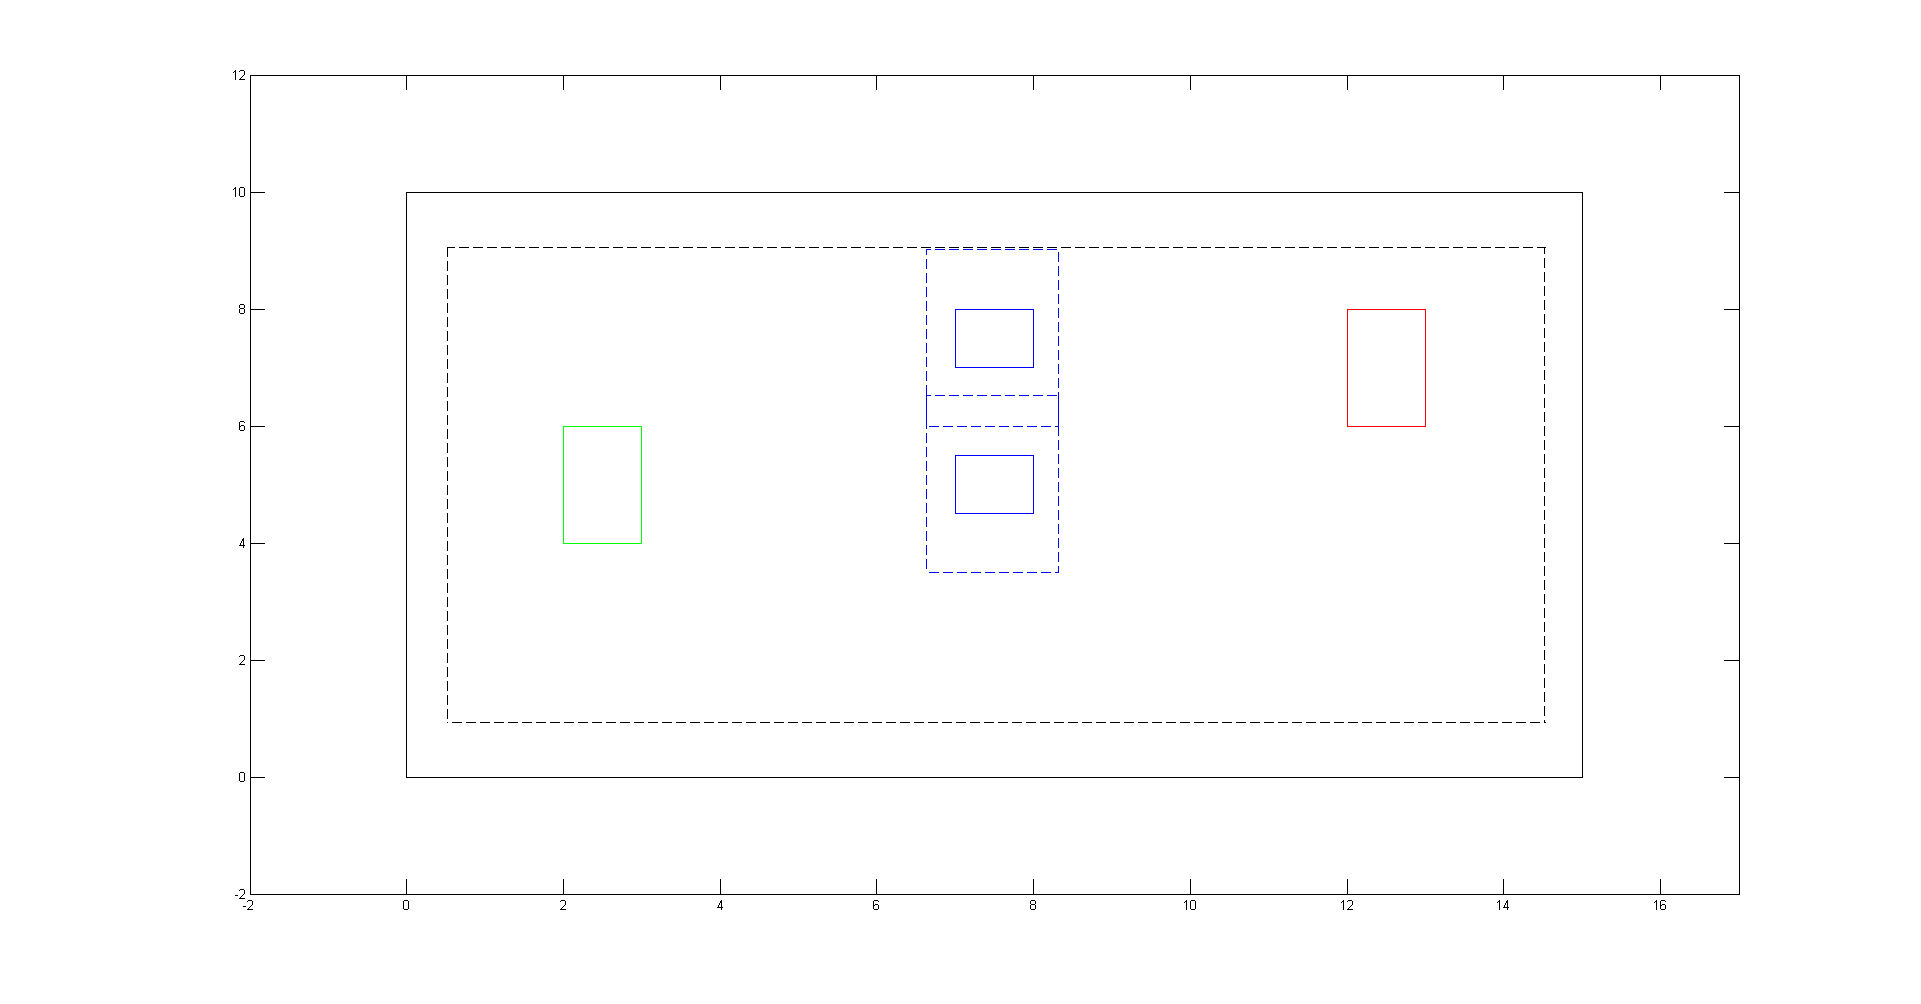
\includegraphics[scale=0.1]{../thesis/riddleWHull}
%\end{figure}
%\end{frame}

\begin{frame}
\frametitle{Kollisionsberechnung mittels Konvexer Hülle II}
Der Vektor bestehend aus der Objektmitte als Aufpunkt und dem Richtungsvektor der Bewegung wird nun auf Schnittpunkte mit den Berechneten Vektoren der Konvexen Hüllen überprüft.
\begin{figure}
\centering
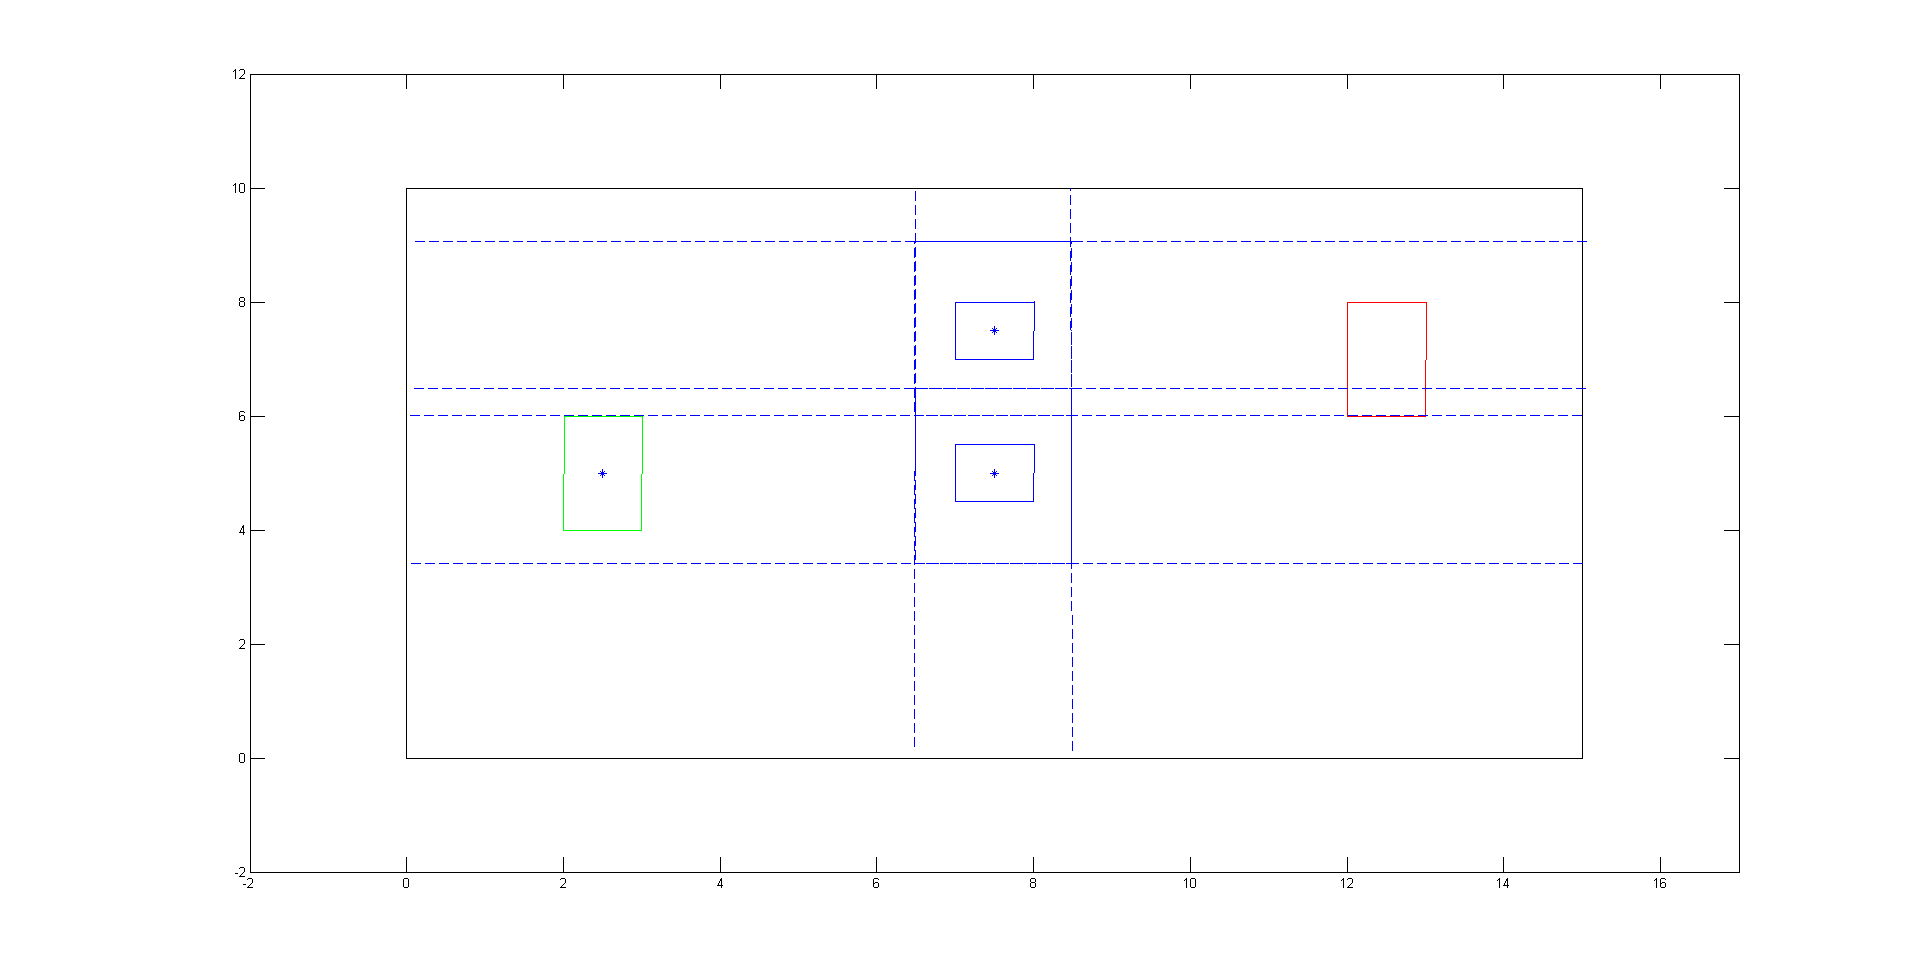
\includegraphics[scale=0.1]{../thesis/riddle2HullCell}
\end{figure}
\end{frame}

\begin{frame}
\frametitle{Auswirkungen von Rotation}
Rotationen erhöhen die Anzahl an Kanten der Konvexen Hüllen.
\begin{figure}
\centering
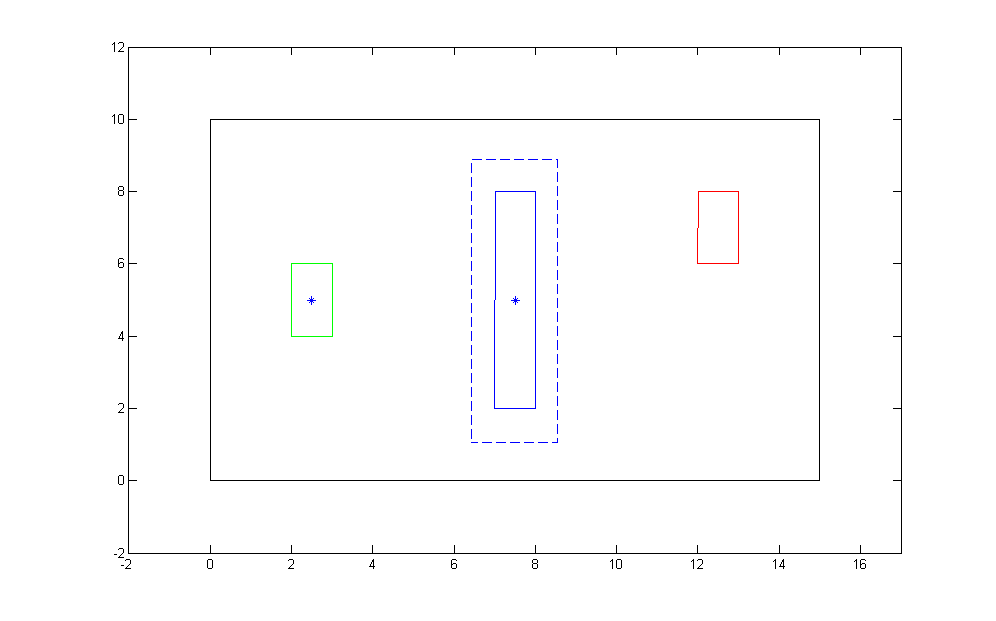
\includegraphics[scale=0.2]{../thesis/rotHull}
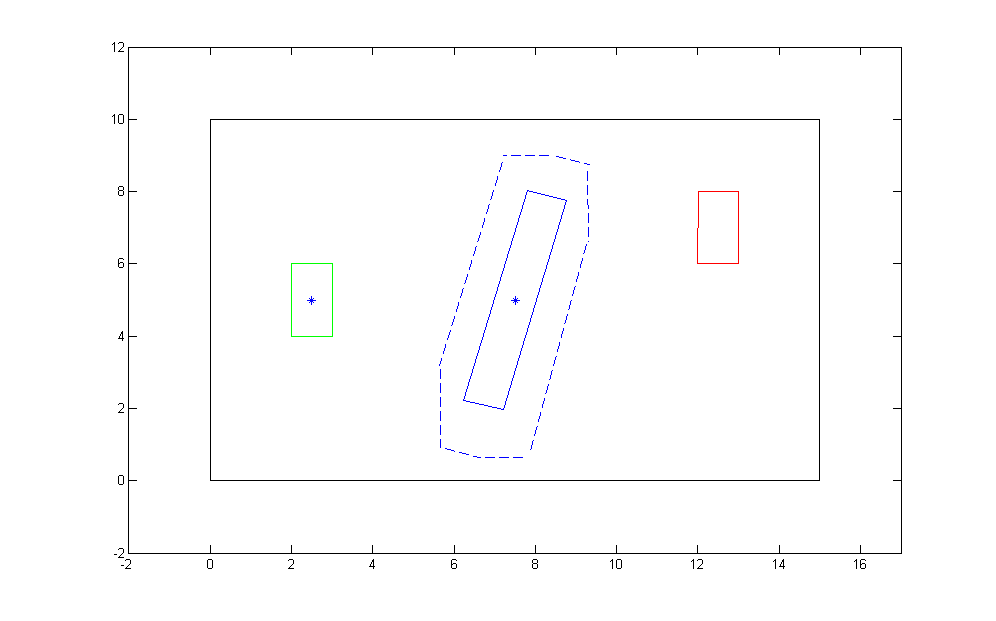
\includegraphics[scale=0.2]{../thesis/rotatedHull}
\end{figure}
\end{frame}



\begin{frame}
\frametitle{Lösungsweg am Beispiel}
Lösung eines Rätsels mit Vektorrepräsentation und Zelleinteilung\\
\begin{figure}
\centering
\movie[externalviewer]{ 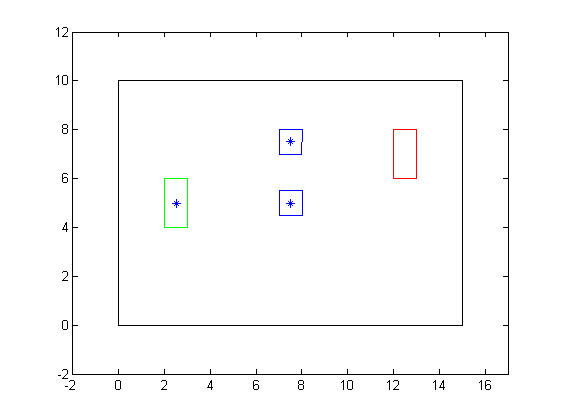
\includegraphics[scale=0.3]{../thesis/riddle2}}{../vectorPath.avi}
\end{figure}
%\includemedia[activate = pageopen , addresource=../vectorPath.mp4, flashvars={source=../vectorPaths.mp4}]{ }{../vectorPath.mp4}
\end{frame}

\section{Kantenrepräsentation mit Funktionen}

\begin{frame}
\frametitle{Kanten als Funktionen}
Bei der Erstellung der Objekte werden nicht Eckpunkte, sondern Funktionen und Definitionsbereiche festgelegt.
\end{frame}

\begin{frame}
\frametitle{Kollisionsberechnung mittels Funktionen}
Kollision ist nun durch das finden von Schnittpunkten zwischen den Funktionen möglich.
Durch Definitionsbereich werden viele Rechnungen stark verkürzt.
\begin{figure}
\centering
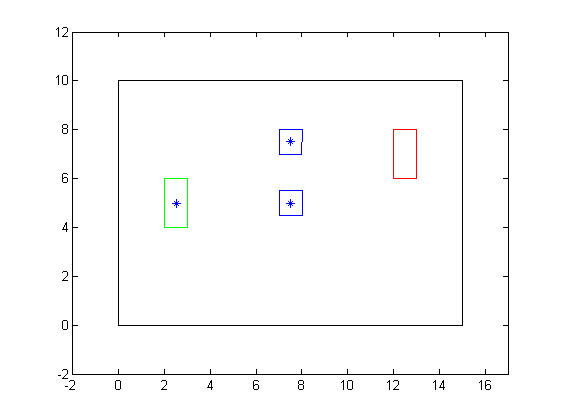
\includegraphics[scale=0.3]{../thesis/riddle2}
\end{figure}
\end{frame}

\begin{frame}
\frametitle{Auswirkungen von Rotation}
Rotationen könnten dazu führen, das eine vertikale Kante mit einer Steigung von unendlich erzeugt wird.
\end{frame}

\begin{frame}
\frametitle{Darstellung von Zellen}
Zellen sind durch die Lage des Objektes zu den Funktionen Definiert.
\begin{figure}
\centering
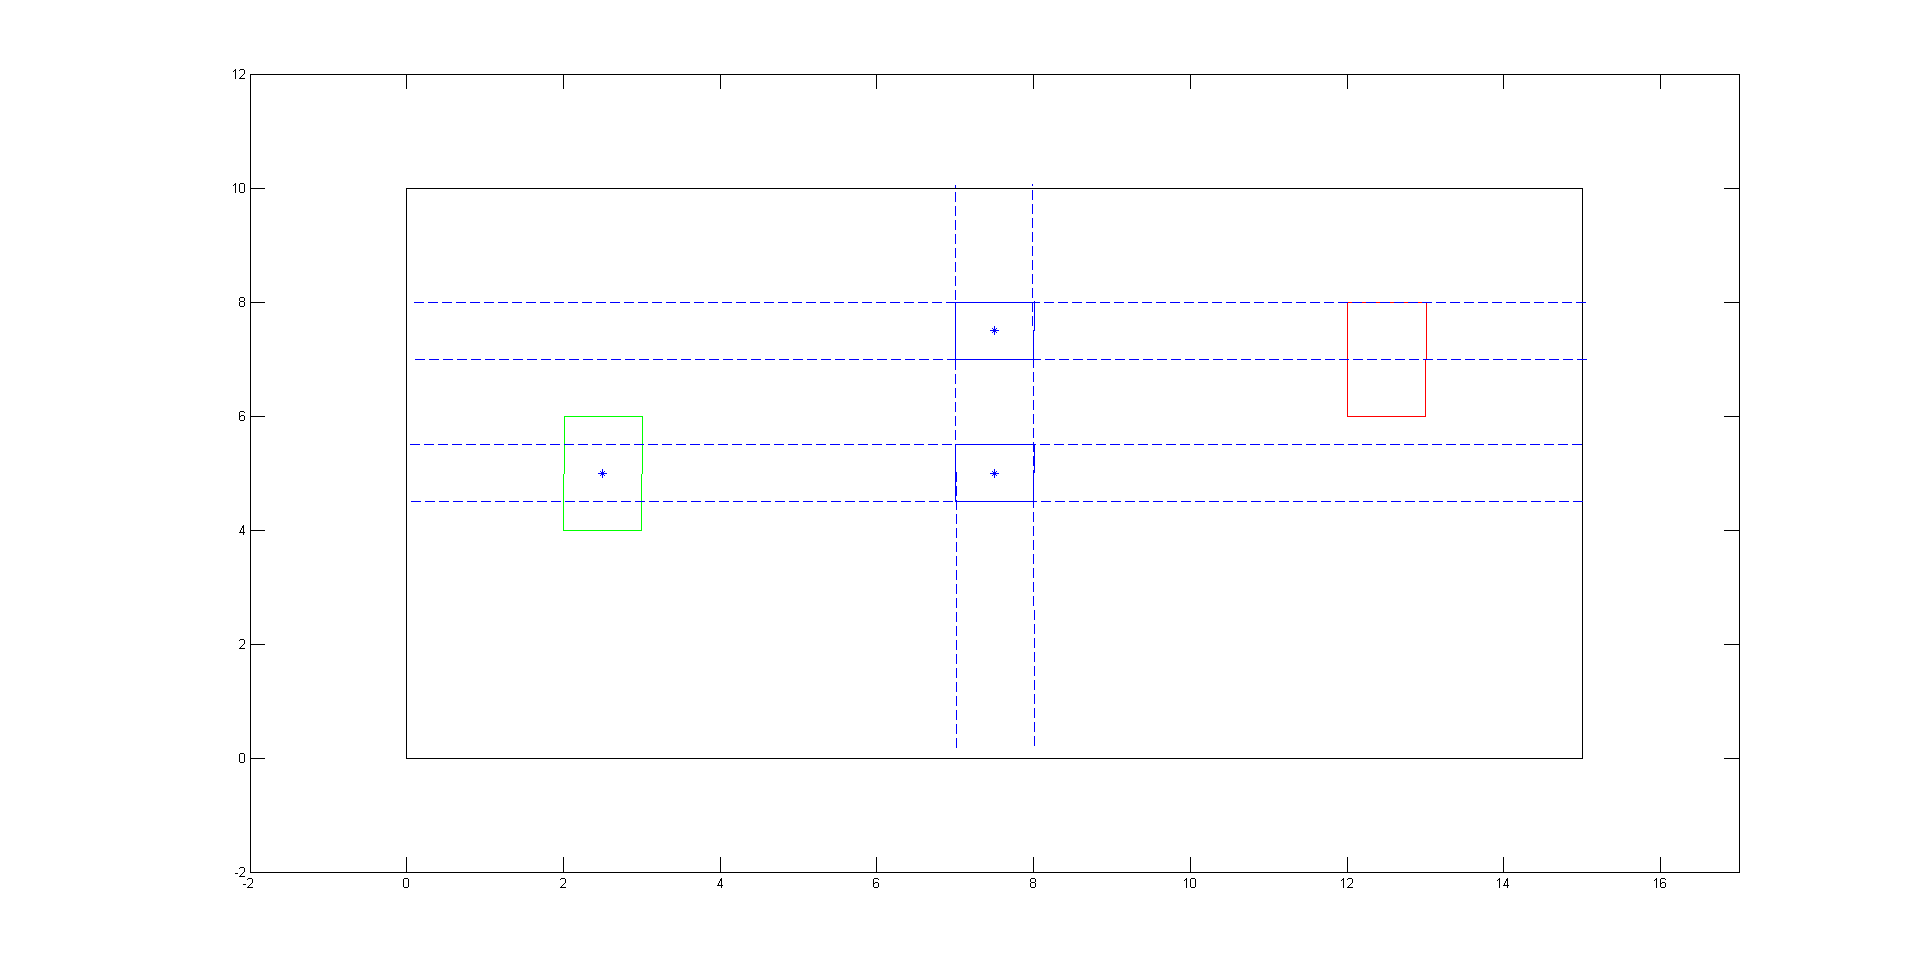
\includegraphics[scale=0.2]{../thesis/riddle2FuncCell}
\end{figure}
\end{frame}

\begin{frame}
\frametitle{Lösungsweg am Beispiel}
Lösung eines Rätsels mit Funktionsrepräsentation ohne Zellen\\
\begin{figure}
\centering
\movie[externalviewer]{ 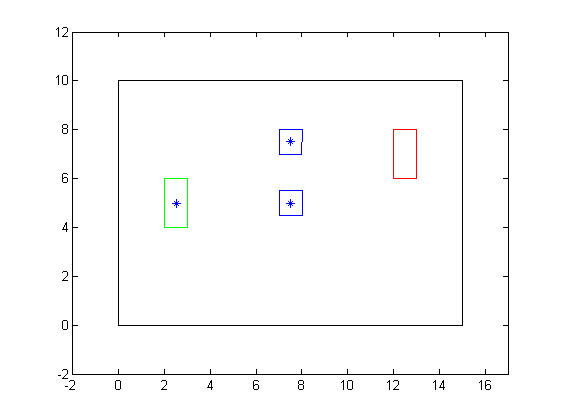
\includegraphics[scale=0.3]{../thesis/riddle2}}{../funcPath.avi}
\end{figure}
%\includemedia[activate = pageopen , addresource=../vectorPath.mp4, flashvars={source=../vectorPaths.mp4}]{ }{../vectorPath.mp4}
\end{frame}

\begin{frame}
\frametitle{Lösungsweg am Beispiel}
Lösung eines Rätsels mit Funktionsrepräsentation mit Zellen\\
\begin{figure}
\centering
\movie[externalviewer]{ 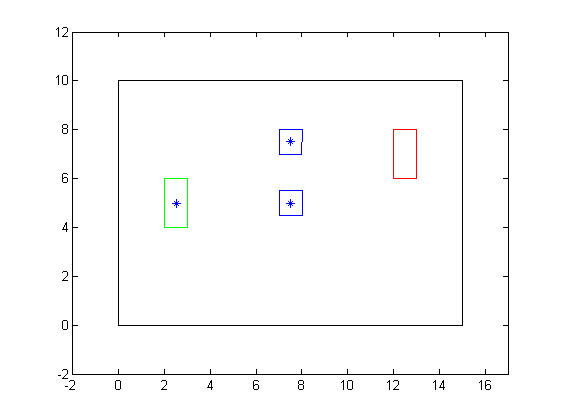
\includegraphics[scale=0.3]{../thesis/riddle2}}{../cellPath.avi}
\end{figure}
%\includemedia[activate = pageopen , addresource=../vectorPath.mp4, flashvars={source=../vectorPaths.mp4}]{ }{../vectorPath.mp4}
\end{frame}

\section{Resultat und Diskussion}

\begin{frame}
Zeiten der verschiedenen implementierten Algorithmen:\\
\vskip 1cm
\begin{tabular}{l||c|c|c|c||}
Algorithmus&2 Objekte&4 Objekte&6 Objekte & 8 Objekte\\\hline\hline
Vector+Zellen &4.9305& 89.3621&403.9329&1855.4 \\
Funktion-Zellen  &0.6747   & 7.7242& 33.7001  & 32.1049 \\
Funktion+Zellen &  0.1472  &13.5623 & 50.3155 & 100.63497\\
\end{tabular}
\end{frame}

\begin{frame}
Benötigte Zeit gegen Objekte im Rätsel
\begin{figure}
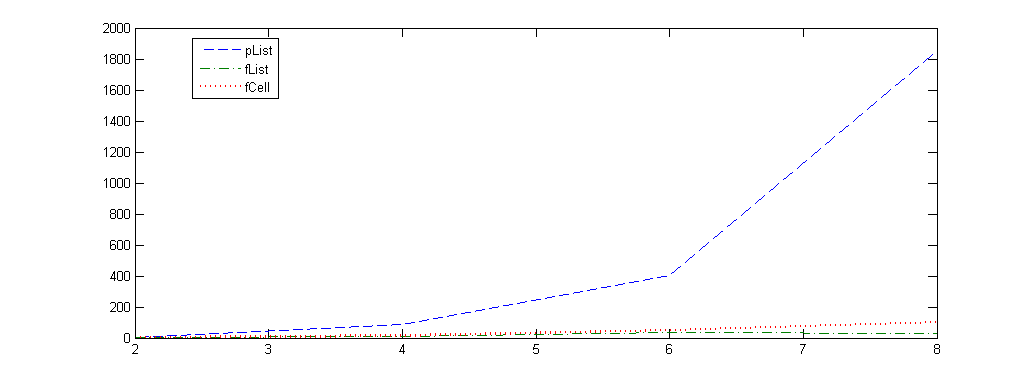
\includegraphics[width=\textwidth]{../thesis/pointAgainstFuncAgainstCell.png}
\end{figure}
\end{frame}

\begin{frame}
''Schlechte'' Rätsel:
\begin{figure}
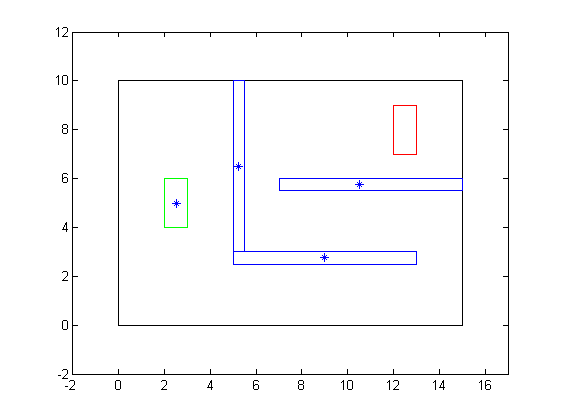
\includegraphics[scale = 0.3]{../thesis/riddleB.png}
\end{figure}
\begin{center}
\begin{tabular}{l||c|c|c||}
& \multicolumn{3}{c||}{6 Objekte} \\\hline\hline
Algorithm& schnellste Zeit & längste  Zeit& mittlere Zeit \\\hline
Funktion-Zellen  &  34234 &  35599 & 34917 \\
Funktion+Zellen & 24.036 & 27.8225 & 25.001 \\
\end{tabular}
\end{center}
\end{frame}

\begin{frame}
Ausblick:
\begin{itemize}
\item Zulassen nicht-konvexer Objekte.
\item Rotation Abschnittsweise als kontinuierliche Funktion definieren.
\item Krumme Oberflächen exakt durch Funktionen Repräsentieren.
\end{itemize}
\end{frame}

\begin{frame}
\begin{center}
Fragen?
\end{center}
\end{frame}

\begin{frame}
\center 
Vielen Dank für Ihre Aufmerksamkeit.
\end{frame}

\end{document}
